\begin{figure}[t]
\centering
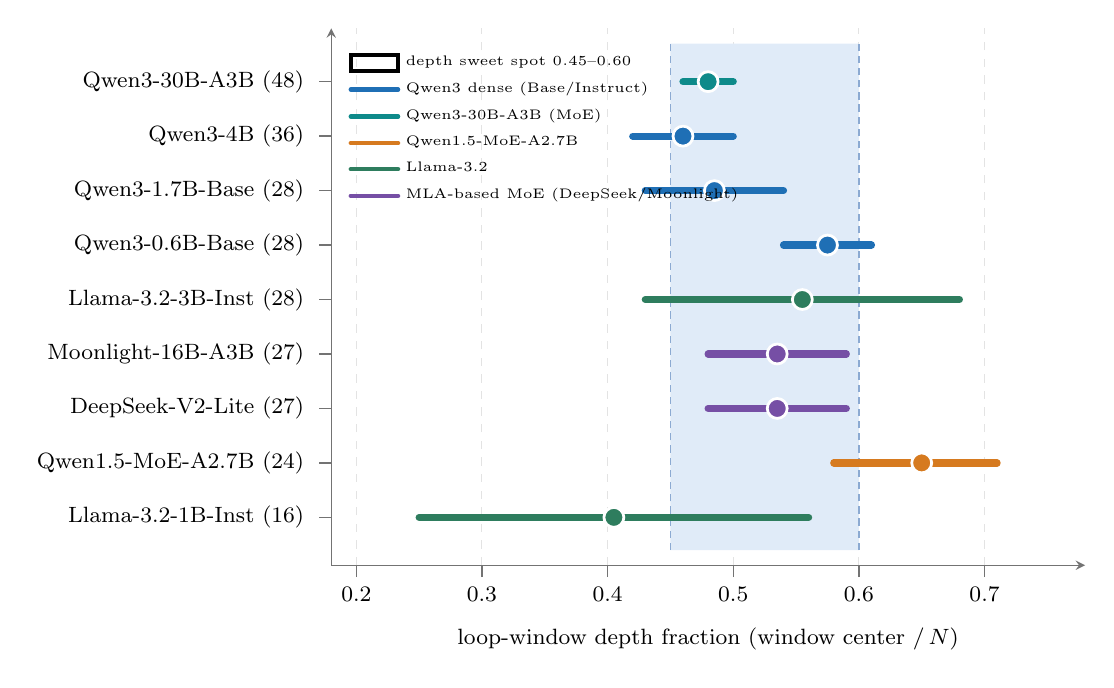
\begin{tikzpicture}
\begin{axis}[
  width=0.92\linewidth,
  height=8.4cm,
  xmin=0.18, xmax=0.78,
  ymin=-0.6, ymax=8.7,
  xtick={0.2,0.3,0.4,0.5,0.6,0.7},
  xticklabel style={font=\footnotesize},
  xlabel={\footnotesize loop-window depth fraction (window center $/\,N$)},
  xlabel style={yshift=-3pt},
  ytick={0,1,2,3,4,5,6,7,8},
  yticklabels={Llama-3.2-1B-Inst (16),
               Qwen1.5-MoE-A2.7B (24),
               DeepSeek-V2-Lite (27),
               Moonlight-16B-A3B (27),
               Llama-3.2-3B-Inst (28),
               Qwen3-0.6B-Base (28),
               Qwen3-1.7B-Base (28),
               Qwen3-4B (36),
               Qwen3-30B-A3B (48)},
  yticklabel style={font=\footnotesize, align=right, xshift=-2pt},
  axis y line=left,
  axis x line=bottom,
  axis line style={line width=0.5pt, draw=black!55},
  enlarge y limits=0.03,
  major grid style={dashed, gray!22, line width=0.35pt},
  xmajorgrids=true,
  tick align=outside,
  tick style={black!55, line width=0.5pt},
  legend style={font=\tiny, draw=none,
                at={(0.015,0.97)}, anchor=north west, fill=none,
                inner sep=2pt, row sep=0.5pt,
                fill opacity=0, text opacity=1},
  legend columns=1,
  legend cell align=left,
  legend image post style={line width=1.6pt, line cap=round},
  clip=false,
]

\addplot[fill={rgb,255:red,224;green,235;blue,248},
         draw=none, area legend]
  coordinates {(0.45,-0.6) (0.60,-0.6) (0.60,8.7) (0.45,8.7)}
  \closedcycle;
\addlegendentry{depth sweet spot $0.45$--$0.60$}

\draw[draw={rgb,255:red,140;green,170;blue,210}, line width=0.55pt,
      dash pattern=on 2.6pt off 1.8pt]
  (axis cs:0.45,-0.6) -- (axis cs:0.45,8.7);
\draw[draw={rgb,255:red,140;green,170;blue,210}, line width=0.55pt,
      dash pattern=on 2.6pt off 1.8pt]
  (axis cs:0.60,-0.6) -- (axis cs:0.60,8.7);

\addlegendimage{line width=2.4pt, line cap=round,
                color={rgb,255:red,31;green,111;blue,181}}
\addlegendentry{Qwen3 dense (Base/Instruct)}

\addlegendimage{line width=2.4pt, line cap=round,
                color={rgb,255:red,14;green,138;blue,138}}
\addlegendentry{Qwen3-30B-A3B (MoE)}

\addlegendimage{line width=2.4pt, line cap=round,
                color={rgb,255:red,214;green,122;blue,31}}
\addlegendentry{Qwen1.5-MoE-A2.7B}

\addlegendimage{line width=2.4pt, line cap=round,
                color={rgb,255:red,46;green,125;blue,94}}
\addlegendentry{Llama-3.2}

\addlegendimage{line width=2.4pt, line cap=round,
                color={rgb,255:red,118;green,79;blue,165}}
\addlegendentry{MLA-based MoE (DeepSeek/Moonlight)}

\draw[draw={rgb,255:red,46;green,125;blue,94}, line width=2.6pt,
      line cap=round] (axis cs:0.25,0) -- (axis cs:0.56,0);
\addplot[mark=*, mark size=3.6pt,
         mark options={fill={rgb,255:red,46;green,125;blue,94},
                       draw=white, line width=1.0pt},
         only marks, forget plot] coordinates {(0.405,0)};

\draw[draw={rgb,255:red,214;green,122;blue,31}, line width=2.6pt,
      line cap=round] (axis cs:0.58,1) -- (axis cs:0.71,1);
\addplot[mark=*, mark size=3.6pt,
         mark options={fill={rgb,255:red,214;green,122;blue,31},
                       draw=white, line width=1.0pt},
         only marks, forget plot] coordinates {(0.65,1)};

\draw[draw={rgb,255:red,118;green,79;blue,165}, line width=2.6pt,
      line cap=round] (axis cs:0.48,2) -- (axis cs:0.59,2);
\addplot[mark=*, mark size=3.6pt,
         mark options={fill={rgb,255:red,118;green,79;blue,165},
                       draw=white, line width=1.0pt},
         only marks, forget plot] coordinates {(0.535,2)};

\draw[draw={rgb,255:red,118;green,79;blue,165}, line width=2.6pt,
      line cap=round] (axis cs:0.48,3) -- (axis cs:0.59,3);
\addplot[mark=*, mark size=3.6pt,
         mark options={fill={rgb,255:red,118;green,79;blue,165},
                       draw=white, line width=1.0pt},
         only marks, forget plot] coordinates {(0.535,3)};

\draw[draw={rgb,255:red,46;green,125;blue,94}, line width=2.6pt,
      line cap=round] (axis cs:0.43,4) -- (axis cs:0.68,4);
\addplot[mark=*, mark size=3.6pt,
         mark options={fill={rgb,255:red,46;green,125;blue,94},
                       draw=white, line width=1.0pt},
         only marks, forget plot] coordinates {(0.555,4)};

\draw[draw={rgb,255:red,31;green,111;blue,181}, line width=2.6pt,
      line cap=round] (axis cs:0.54,5) -- (axis cs:0.61,5);
\addplot[mark=*, mark size=3.6pt,
         mark options={fill={rgb,255:red,31;green,111;blue,181},
                       draw=white, line width=1.0pt},
         only marks, forget plot] coordinates {(0.575,5)};

\draw[draw={rgb,255:red,31;green,111;blue,181}, line width=2.6pt,
      line cap=round] (axis cs:0.43,6) -- (axis cs:0.54,6);
\addplot[mark=*, mark size=3.6pt,
         mark options={fill={rgb,255:red,31;green,111;blue,181},
                       draw=white, line width=1.0pt},
         only marks, forget plot] coordinates {(0.485,6)};

\draw[draw={rgb,255:red,31;green,111;blue,181}, line width=2.6pt,
      line cap=round] (axis cs:0.42,7) -- (axis cs:0.50,7);
\addplot[mark=*, mark size=3.6pt,
         mark options={fill={rgb,255:red,31;green,111;blue,181},
                       draw=white, line width=1.0pt},
         only marks, forget plot] coordinates {(0.46,7)};

\draw[draw={rgb,255:red,14;green,138;blue,138}, line width=2.6pt,
      line cap=round] (axis cs:0.46,8) -- (axis cs:0.50,8);
\addplot[mark=*, mark size=3.6pt,
         mark options={fill={rgb,255:red,14;green,138;blue,138},
                       draw=white, line width=1.0pt},
         only marks, forget plot] coordinates {(0.48,8)};

\end{axis}
\end{tikzpicture}
\caption{\textbf{The depth-fraction rule across nine architectures.}
For each checkpoint we plot the best loop-window range $[a/N,\,b/N]$ as a horizontal bar with the window's center $(a{+}b)/(2N)$ as a filled circle. The shaded band marks the 0.45--0.60 depth fraction, which contains 7 of 9 checkpoints' optimal window centers---Qwen3 dense (0.6B--4B), Qwen3-30B-A3B MoE,DeepSeek-V2-Lite, Moonlight-16B-A3B, and Llama-3.2-3B---with only the
sub-1B distilled Llama-3.2-1B (shifted earlier) and the older Qwen1.5-MoE-A2.7B (shifted later) outside.}
\label{fig:depth-rule}
\end{figure}
